%second chapter of your thesis
\chapter{Moeilijkheden}\label{Moeilijkheden}
\section{Software}
Het probleem met de integrator is iets waar we niet dieper op ingegaan zijn en niet hebben opgelost. Het probleem dat zich voordoet is het feit dat de I-waarde die we genereren, telkens de som is van de fout die zich voordoet. Aangezien de code honderden keren per seconde wordt uitgevoerd kan deze waarde in een mum van tijd een extreem grote waarde aannemen wat niet gunstig is voor de robot. Het effect van dit probleem op onze robot was dat hij plots extreem versnelde en onmiddellijk alle controle verloor. We zouden dit probleem kunnen oplossen door de KI-waarde voldoende klein te kiezen en eventueel slechts om de zoveel tijd de I-waarde aan te passen. Na herhaaldelijke pogingen om dit probleem op te lossen hebben we ingezien dat de I-waarde geen noodzakelijk onderdeel is voor een stabiel rijdende robot en hebben we dus besloten deze term weg te laten.

Op het moment dat we onze PD-waarden aan het optimaliseren waren, is er een kortsluiting ontstaan in onze Arduino en motor shield terwijl de batterij aangesloten was. De batterij heeft toen een te grote stroom door beide printplaten gestuurd waardoor deze stuk gingen. Ook 3 sensoren gingen toen in rook op. We hebben toen een hele middag gezocht of er een mogelijkheid was om alsnog de motorshield te herstellen aangezien er geen werkende shields op overschot waren. Jammer genoeg was het de L298 die stuk was en hebben we dan een motor shield gekregen waarbij het kroonsteentje stuk was. Na een kleine opknapbeurt hadden we opnieuw een werkende motorshield ter onze beschikking. Onze PD-waarden waren door de nieuwe shield niet meer optimaal en waardoor we dus 2 dagen verloren hebben aan dit gebeuren.

Aangezien we gebruik maken van 2 armen voor het detecteren van beide lijnen van het parcours, ontstaat er het probleem dat er 1 arm een hogere prioriteit heeft ten opzichte van de andere arm. De code die we ge\"implementeerd hebben zorgt ervoor dat de rechterarm prioriteit heeft boven de linkerarm aangezien de code voor de rechterarm eerst wordt uitgevoerd. Van zodra er 1 sensor actief is van deze arm, zal de code voor de registratie van de sensoren van de linkerarm zelfs niet meer uitgevoerd worden. Dit heeft er voor gezorgd dat onze robot een voorkeursrichting, namelijk tegenwijzerzin, heeft waarin hij met grotere zekerheid de parcours foutloos zal kunnen afleggen. Wanneer we de buitenbocht volgen, wat meestal het geval is, dan bestaat de kans dat bij een plotse scherpe bocht naar links, de robot onvoldoende corrigeert en daardoor met zowel zijn rechterarm, de buitenlijn detecteert, als met zijn linkerarm, de middellijn. Deze situatie zou tot geen probleem leiden aangezien zijn rechterarm prioritair is en dus de wit-detectie van zijn linkerarm teniet gedaan wordt. Omgekeerd daarentegen, wanneer links de buitenbocht is bijvoorbeeld 010 100, en hij komt met zijn rechterarm op de middellijn terecht, dan zal de robot de verkeerde kant uitschieten aangezien hij met een grote factor wordt gecorrigeerd omdat de sensor die de extreme situatie voorstelt, oplicht. Gelukkig zijn de sensor-armen instelbaar en konden we per circuit de richting en afstand van de armen instellen om zo optimale prestaties te verkrijgen zonder het probleem van prioriteit uit de kant te ruimen. Een mogelijkheid om dit probleem aan te pakken was om bij te houden met een boolean welke arm er actief is en welke arm er net nieuw contact maakt met de witte lijn. De arm die bijvoorbeeld al het langst actief was, kunnen we dan als prioritaire arm beschouwen en elke keer dat we de situatie 000 000 tegenkomen, wat overeenkomt met alle sensoren die zich in het zwart bevinden, kan de prioriteit van de arm opnieuw ingesteld worden.

Voor het eenvoudigste, ovale circuit hadden we onze code geoptimaliseerd op 72. Deze snelheid komt overeen met 0.40 m/s en was een zeer hoge snelheid als je onze robot zag rondrijden. Wanneer we vervolgens het 2e circuit te zien kregen, werd het duidelijk dat de robot dit circuit niet aan deze snelheid zou kunnen afleggen. We verlaagden onze snelheid dan naar 65. Deze snelheidsvermindering ging ook gepaard met nieuwe PD-waarden en we konden met andere woorden opnieuw beginnen met het instellen van de robot. Het probleem waar we nu mee te maken kregen, is dat we een lager vermogen hadden voor de motoren en dus bij sommige grote bulten een duwtje moesten geven om onze robot zijn rit te laten verderzetten. De snelheid opdrijven, zou resulteren in het opnieuw aanpassen van de error values en PD-waarden, waardoor we besloten genoegen te nemen met een snelheid van 0.28 m/s.

Op het moment dat onze printplaat, Arduino gecombineerd met een motor shield, klaar was, wilden we de RFID-lezer connecteren met de Arduino. We stuitten op het probleem dat de RFID-lezer gebruik maakt van de pinnen: 9, 10, 11,12 en 13 terwijl we onze printplaat reeds geroute hadden waarbij de pinnen 11 12 en 13 intern verbonden waren met de L298. Dit vormde een groot probleem aangezien het voor de RFID-lezer niet mogelijk was gebruik te maken van andere pinnen omdat er gebruik gemaakt wordt van SPI. Dit probleem konden we oplossen door onze routing volledig opnieuw te doen waarbij we andere pinnen zouden gebruiken om de L298 aan te sturen. Aangezien daar geen tijd voor was, bedachten we dat we konden gebruik maken van een andere hulp-Arduino die instond voor het lezen van de RFID-tags en voor het verzenden via UART naar de hoofd-Arduino. Deze hoofd-Arduino verloor met als gevolg dus slechts 1 pin, namelijk de RX-pin, aan het lezen van de RFID-tags. Aangezien we voordien reeds een prototype-Arduino gemaakt hadden, konden we deze gebruiken als hulp-Arduino en konden we op het einde van de rit alsnog ons project afronden waarbij we enkel gebruik maakten van zelfgemaakte printplaten.

Wanneer we data via Bluetooth verzonden van de Raspberry Pi naar de Arduino en omgekeerd stootten we op het probleem dat er regelmatig karakters fout waren ontvangen en de communicatie dus niet optimaal was. We hebben vervolgens trachten te achterhalen wat het probleem exact was. We merkten op dat de RX- en TX-pinnen, waaraan wij de Bluetooth module hadden aangesloten, ook rechtstreeks verbonden zijn met de USB-poort. Wanneer we dus met behulp van Serial.println(), data wilden wegschrijven naar de seri"ele monitor, gebeurde dat als het ware op dezelfde datalijn als de data die we ontvingen via de Bluetooth module. We konden dit probleem oplossen door niet langer gebruik te maken van Hardware Serial maar wel door Software Serial waarbij we de pinnen A2 en 2 gebruikten als respectievelijk RX en TX.

\section{Hardware}
We waren er ons van bewust dat het vrijwel onmogelijk was dat onze PCB geen kinderziekten zou vertonen bij ons eerste ontwerp. De problemen kwamen vrijwel onmiddellijk tot uiting bij de L298. Het ground-vlak viel wat groter uit dan door de footprint voorzien was waardoor dit vlak contact maakte met een baan waarover +5V stond en dus eigenlijk kortsluiting vormde. We hebben dit probleem kunnen oplossen door plakband tussen het ground-vlak en de printbaan te kleven om zo het contact te verbreken. Hoewel de oplossing niet ideaal was, waren we hiermee wel geholpen. We hebben dan onmiddellijk de footprint gewijzigd zodat onze finale PCB dit probleem niet zou vertonen. We hadden ook problemen met de reset-knop waarbij de afmetingen van de gebruikte footprint niet klopten. We hebben dit opgelost door gebruik te maken van een drukknop met slechts twee pinnen die verbonden worden met elkaar bij het indrukken van de knop. 


Bij het testen van de PCB merkten we vrijwel onmiddellijk op dat een paar componenten warm werden. Dit was een directe indicatie van het feit dat de printplaat nog niet op punt stond. We hebben na lang zoeken en met hulp van onze coach, 3 problemen ontdekt. We hebben deze problemen ook aangeduid op figuren~\ref{fig:prob1} en~\ref{fig:prob3}.
Probleem 1 was een Schottky-diode die niet goed verbonden was met zijn baantje. De diode maakte soms wel contact en soms niet. Daar de footprint van de diode nog steeds te klein uitviel hebben we het probleem opgelost door een draadje te solderen aan de contactzijde om zo een verbinding te maken met de baan.
Probleem 2 was simpelweg een via die we over het hoofd gezien hadden waardoor een pin van de L298 niet verbonden was. 
Probleem 3 was de grootste boosdoener. We waren in het schema \'e\'en label vergeten te plaatsen waardoor de L298, die in staat voor de motorsturing, niet gevoed werd met PWRIN. Hierdoor werden de signalen niet goed verwerkt door de L298 en kregen de motoren dus ook niet de juiste signalen. We hebben dit nogmaals opgelost door een verbinding te solderen tussen de IC en de PWRIN. De PWRIN is het signaal dat rechtstreeks via de kroonsteentjes binnenkomt van de batterij.
\begin{figure}[h]
\centering
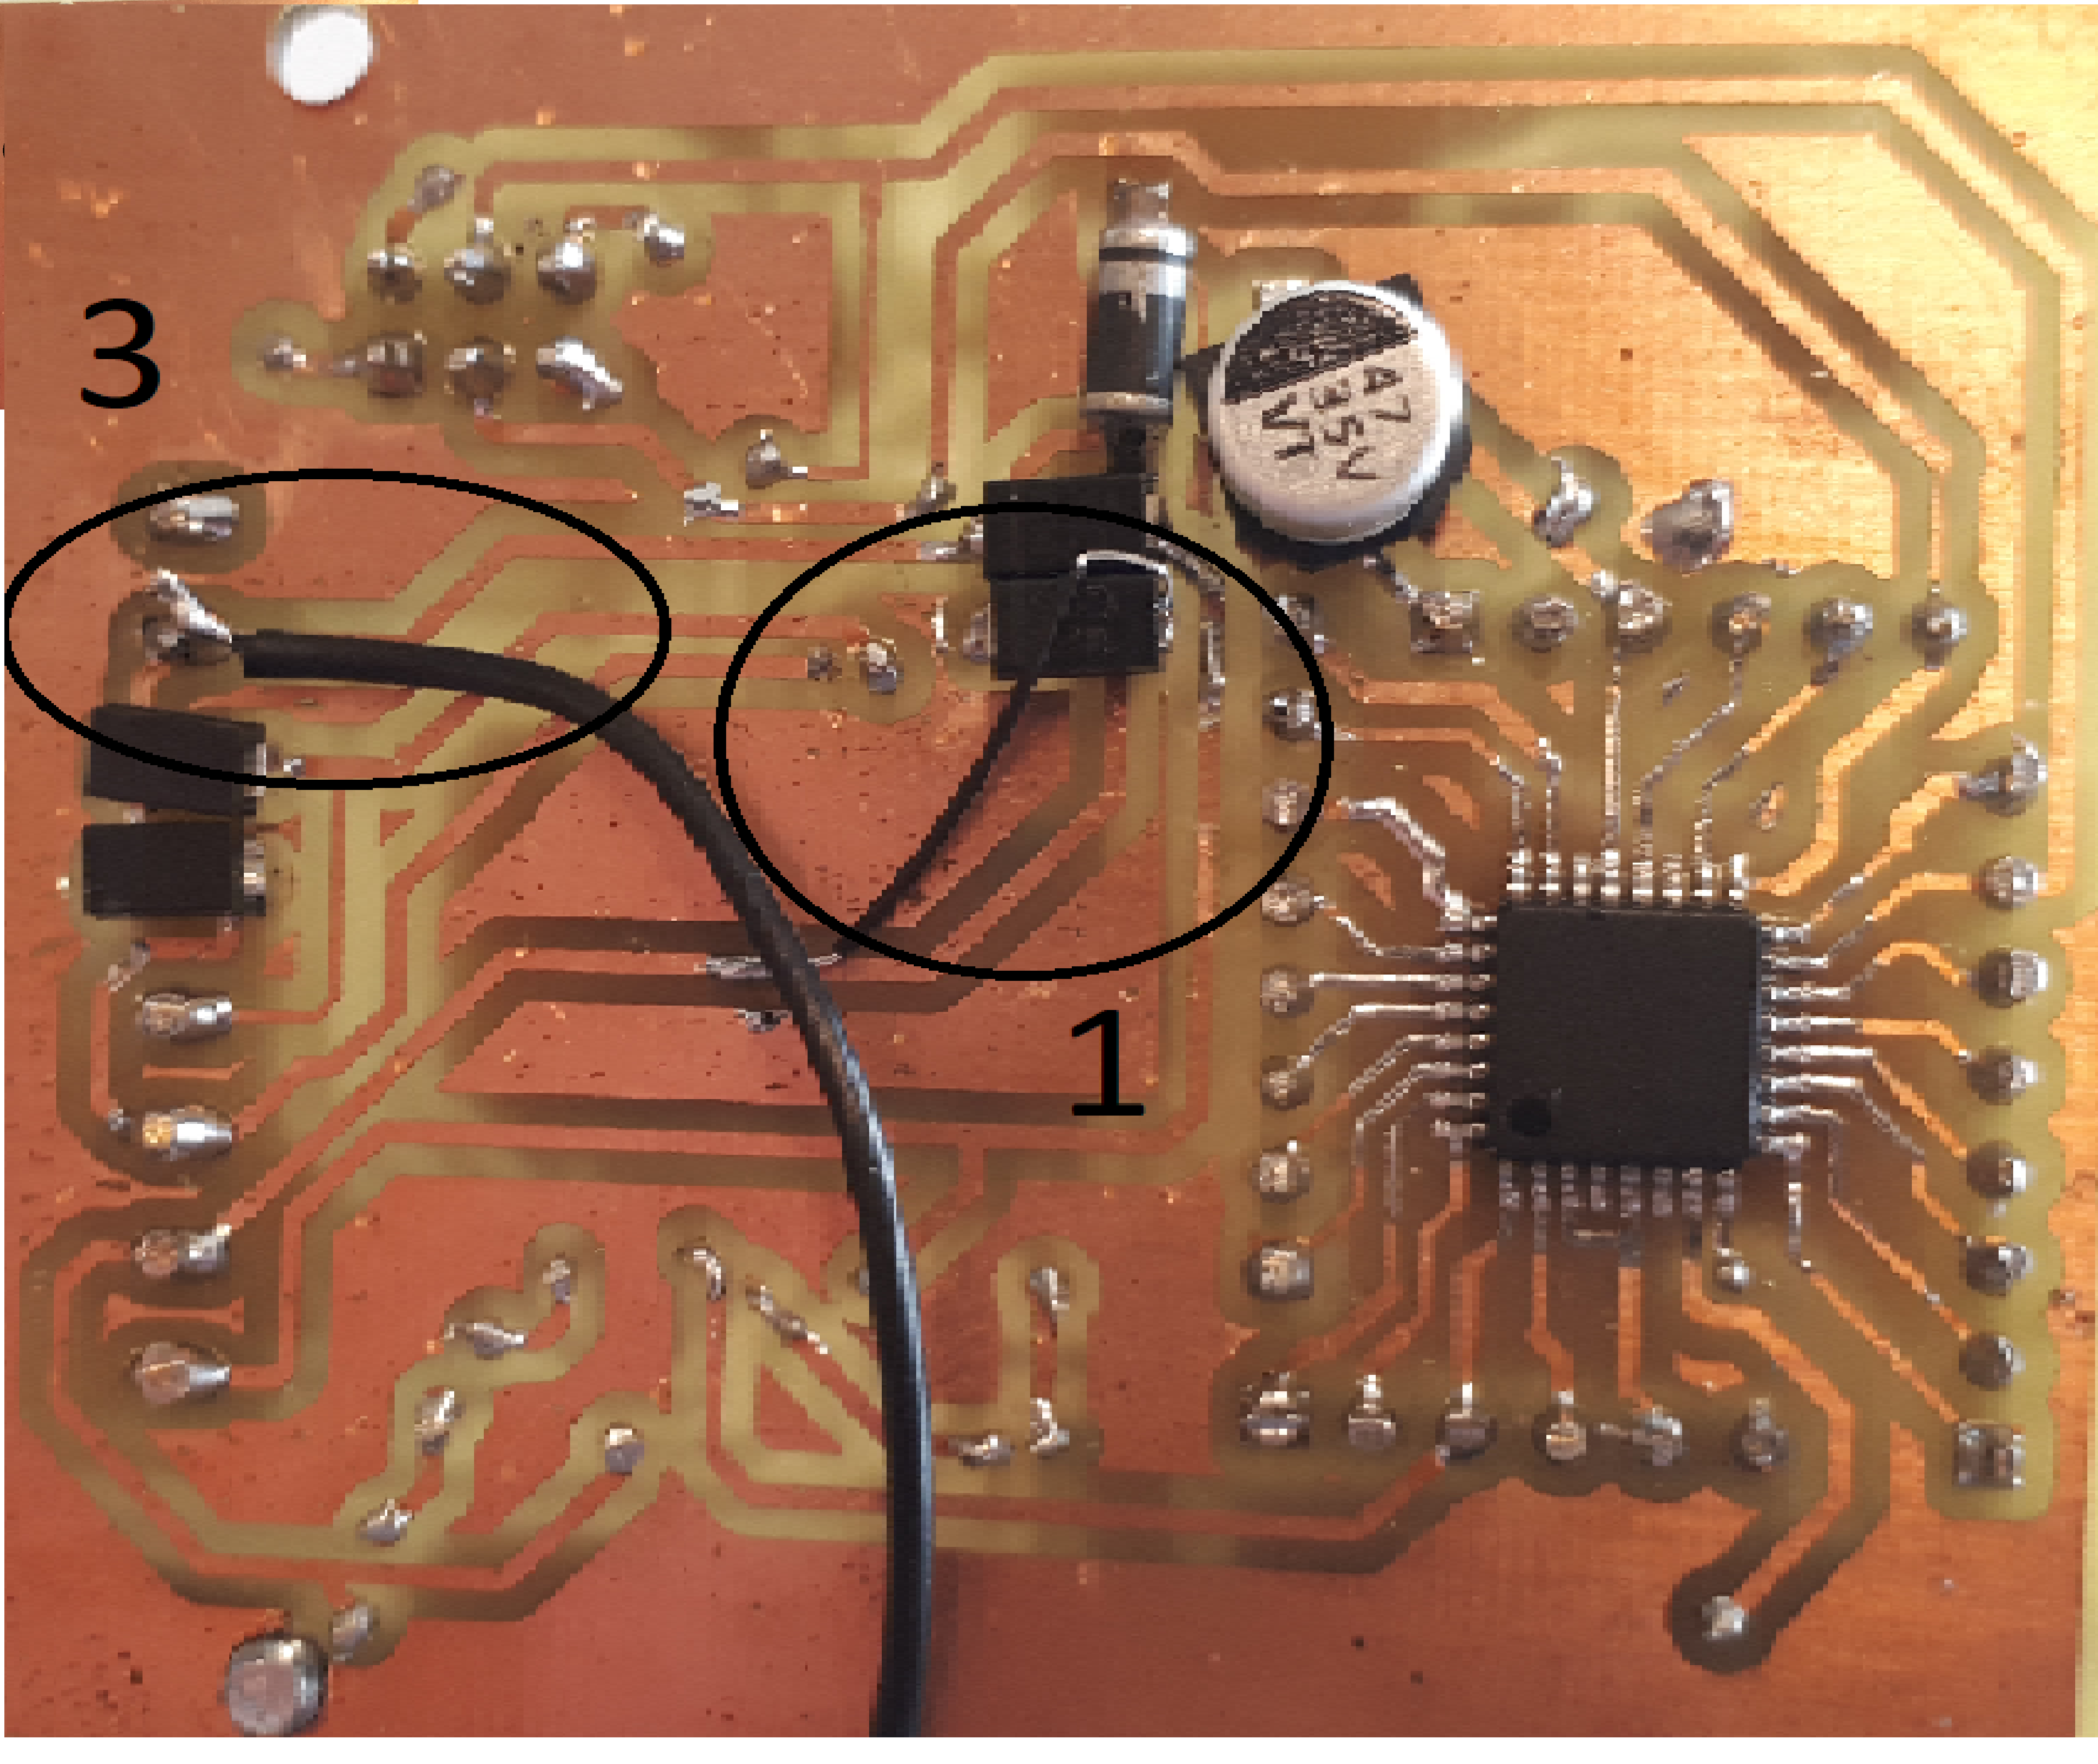
\includegraphics[width=0.25\textwidth]{PCBProblemenVoorkant.png}
\caption{Probleem 1 en 3 bij het PCB ontwerp}
\label{fig:prob1}
\end{figure}

\begin{figure}[h]
\centering
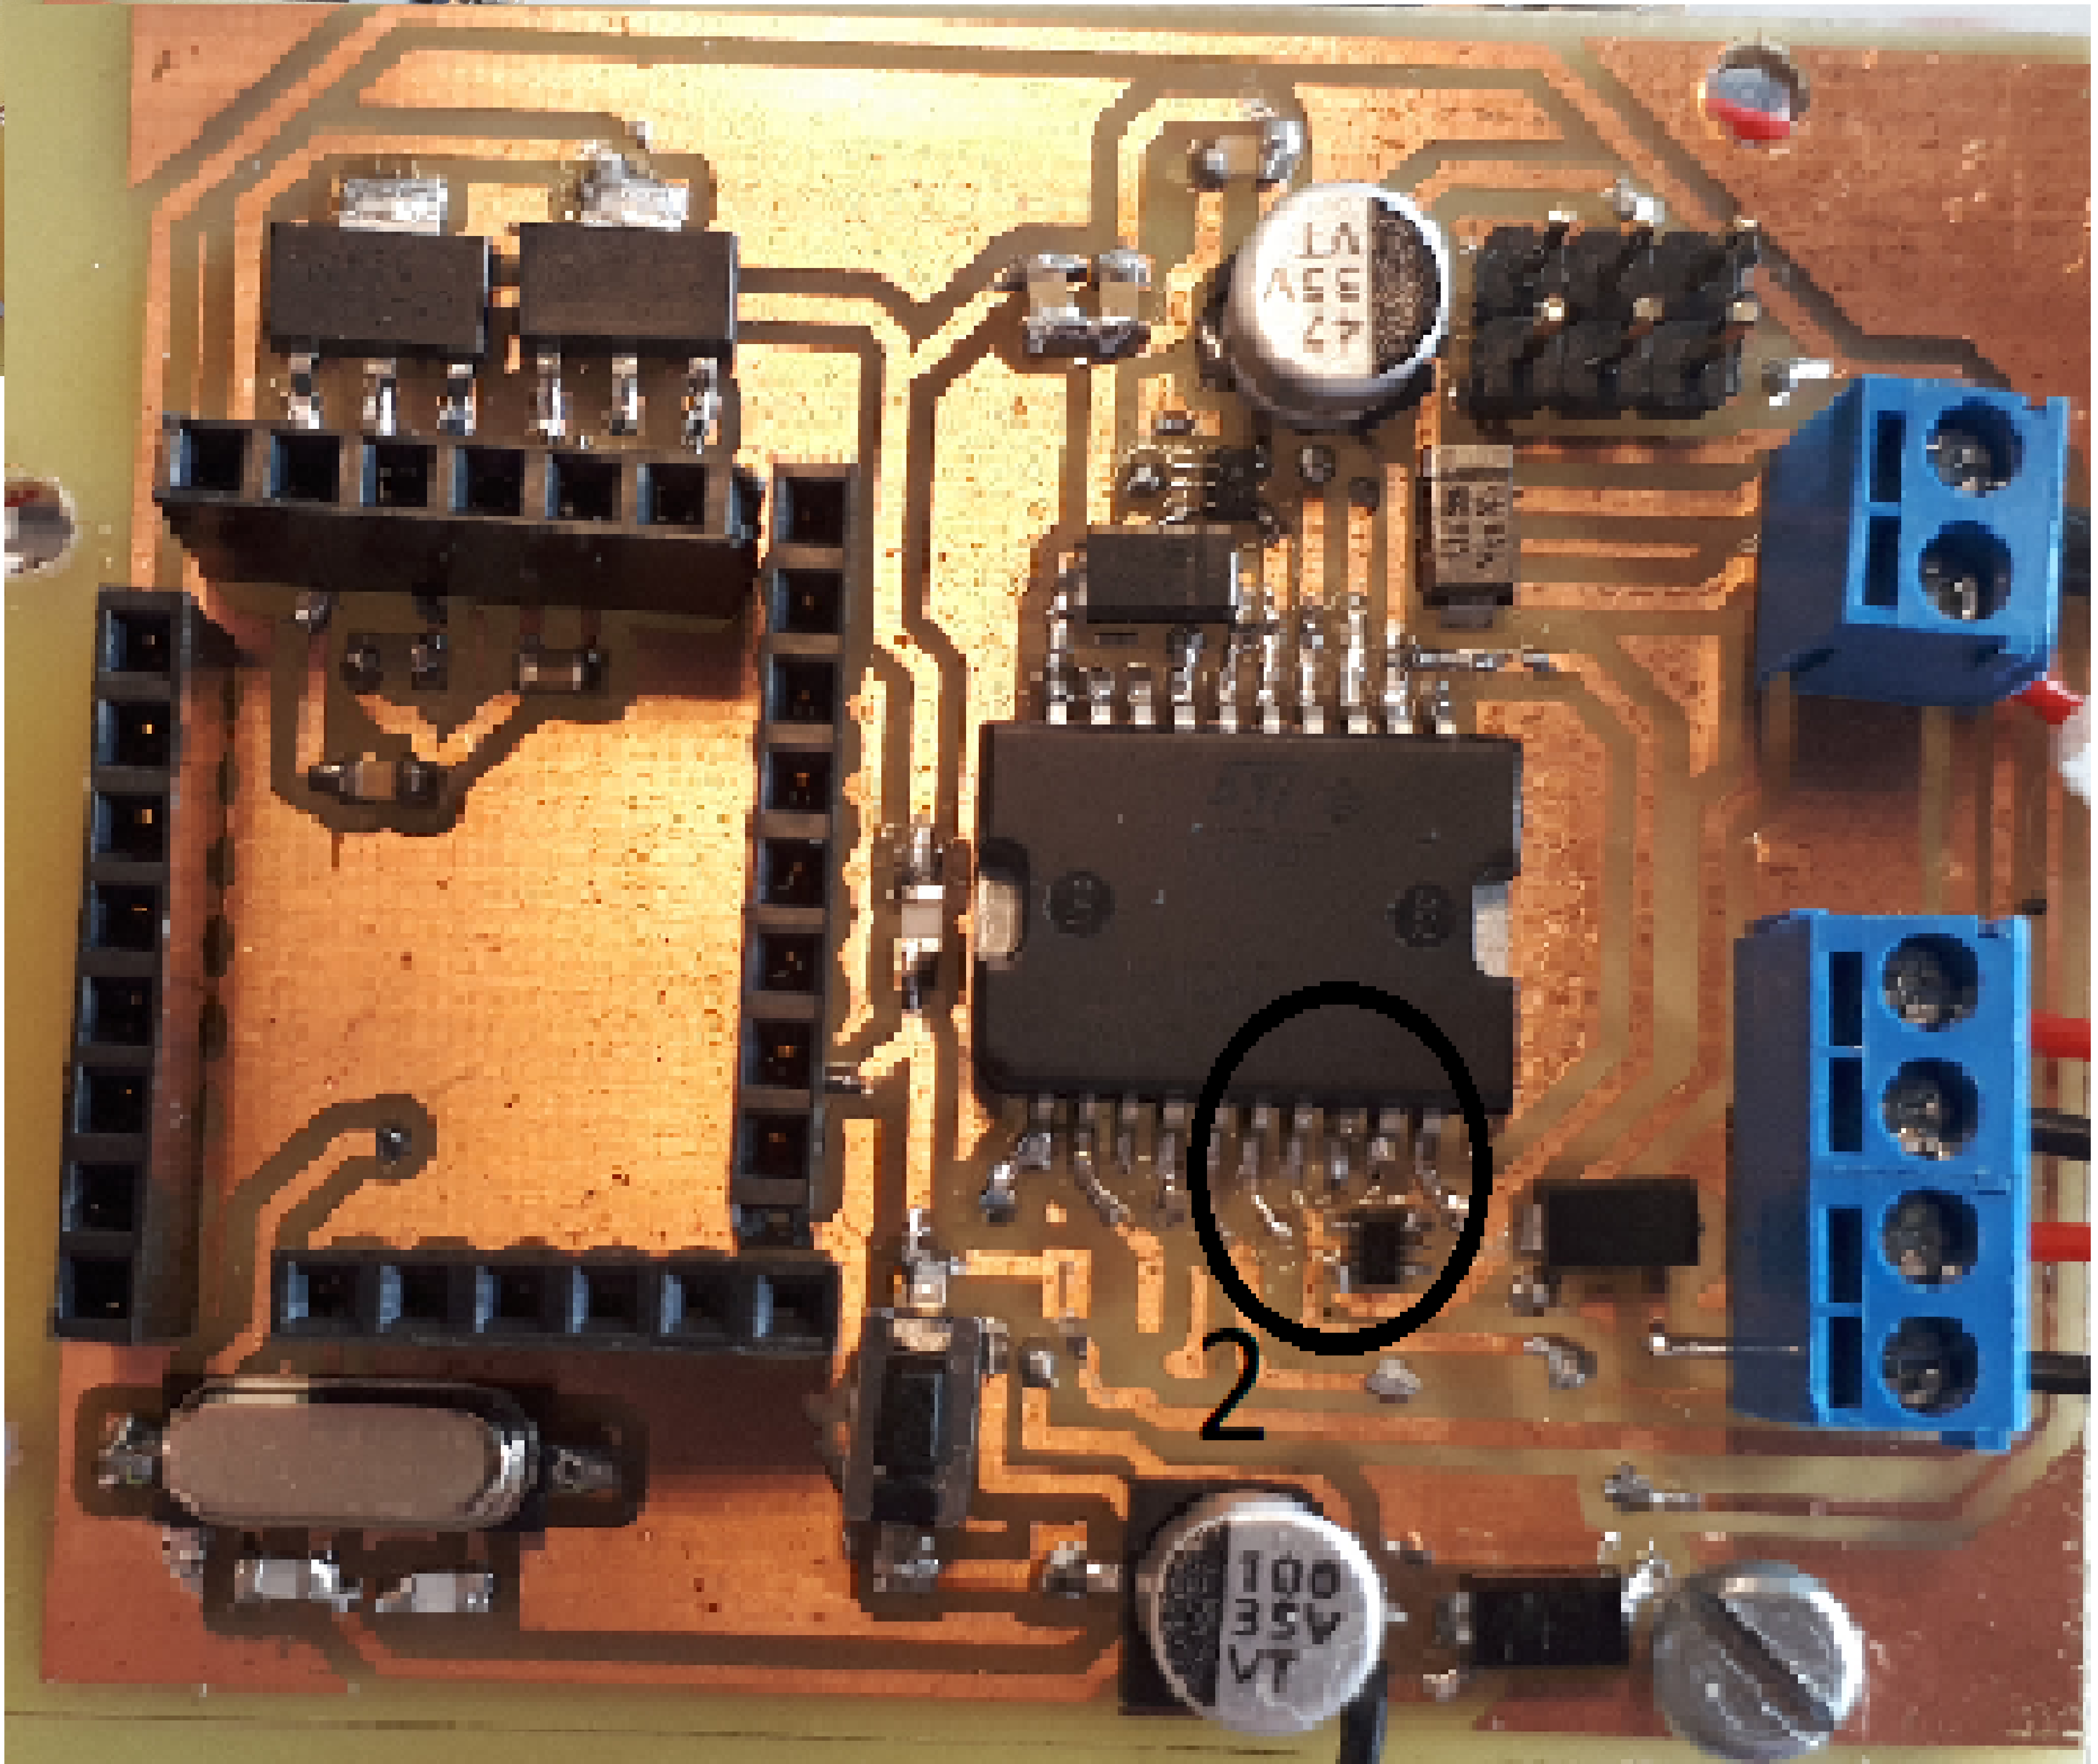
\includegraphics[width=0.25\textwidth]{PCBProblemenAchterkant.png}
\caption{Probleem 2 bij het PCB ontwerp}
\label{fig:prob3}
\end{figure}



